\documentclass[12pt,a4paper]{report}
\usepackage[utf8]{inputenc}
\usepackage[french]{babel}
\usepackage{csquotes}
\usepackage[T1]{fontenc}
\usepackage{amsmath}
\usepackage{amsfonts}
\usepackage{amssymb}
\setcounter{secnumdepth}{3}
\usepackage{lmodern}
\usepackage[protrusion=true,expansion=true]{microtype}
\usepackage{setspace}
\usepackage[Genny]{fncychap}
\newtheorem{propriete}{Propriété}[section]
\usepackage{fancyhdr}
\usepackage{fancybox}
\linespread{1.5}
\usepackage{setspace}
\usepackage{enumerate}
\usepackage{lastpage}
\pagestyle{fancy}
\fancyhf{}
\renewcommand{\headrulewidth}{0pt}
\usepackage{multirow}
\usepackage{lipsum}
\usepackage{etoc}
\usepackage[left=1.5cm, right=1.5cm,bottom=1.5cm,top=1cm]{geometry}
\usepackage{tcolorbox}
\usepackage{graphicx}
\usepackage{tikz}
\usetikzlibrary{positioning, calc}
\definecolor{mycolor}{HTML}{054919}
\definecolor{moncolor}{HTML}{f7e50c}
\usepackage{siunitx}
\usepackage{float}
\usepackage{tabularray}
\UseTblrLibrary{amsmath,booktabs,counter,diagbox,siunitx,varwidth}
\usepackage{tocloft}
\usepackage[french]{babel}

\usepackage{titlesec}  % Package pour personnaliser les titres

\bibliographystyle{plainnat}  % Style numérique
\usepackage[backend=bibtex]{biblatex}  % Utilise biblatex pour la gestion de bibliographie
\addbibresource{Références.bib}        % Charge ton fichier .bib

\titleformat{\chapter}[hang] % Formater le titre des chapitres
{\normalfont\LARGE\bfseries}  % Style du texte (gros et en gras)
{Chapitre \thechapter{} :}    % Ajouter "Chapitre" suivi du numéro en chiffre romain
{20pt}                        % Espace entre "Chapitre X :" et le titre
{\LARGE\bfseries}             % Style du titre du chapitre
\renewcommand{\thechapter}{\Roman{chapter}}  % Numérotation des chapitres en chiffres romains


\begin{document}
	\renewcommand{\tablename}{Tableau}
	
	\newcommand{\innerMargin}{0.5cm}
	\begin{tikzpicture}[remember picture, overlay]
		\draw[
		line width=3pt,
		color=mycolor,
		]
		([xshift=\innerMargin, yshift=-\innerMargin]current page.north west)
		rectangle
		([xshift=-\innerMargin, yshift=\innerMargin]current page.south east);
	\end{tikzpicture}
	
	\noindent
	\pagestyle{empty}
	
	\begin{minipage}[t]{0.45\textwidth}
		\fontsize{10pt}{0.45cm}\selectfont
		\begin{center}
			MINISTERE DE L'ENSEIGNEMENT SUPERIEUR, DE LA RECHERCHE ET DE L'INNOVATION\\
			- - - - - - - - - - - - - - \\
			SECRETARIAT GENERAL\\
			- - - - - - - - - - - - - - \\
			DIRECTION GENERALE DE L’ENSEIGNEMENT SUPERIEUR\\
			- - - - - - - - - - - - - - - - - - \\
			INSTITUT SUPERIEUR DES FILIERES PROFESSIONNALISANTES \vspace*{0.7cm}
			
			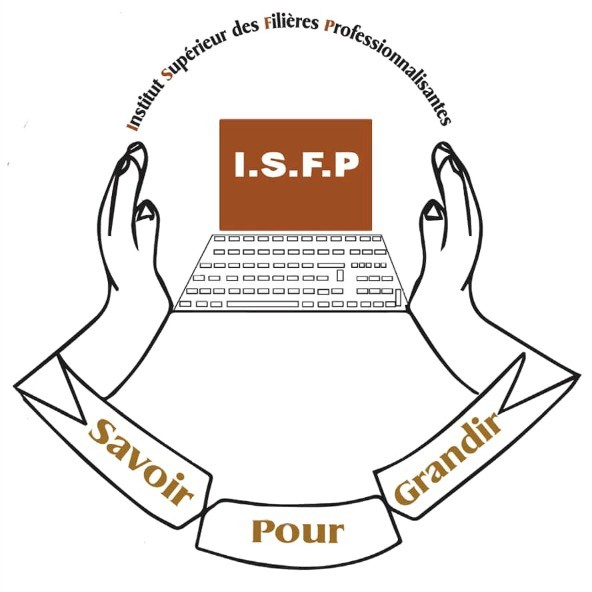
\includegraphics[scale=0.18]{isfp.png}\\
			\textbf{\small 01 BP 1496 Bobo 01} \\[-1ex]
			\textbf{\small E-mail : isfpburkina@yahoo.fr} \\[-1ex]
			\textbf{\small Site web : www.isfpburkina.org} \\[-1ex]
			\textbf{\small Tel : +226 20 97 54 56} \\	
		\end{center}	
	\end{minipage}
	\hspace{0.1\textwidth}
	\noindent
	\begin{minipage}[t]{0.4\textwidth}
		\fontsize{10pt}{0.4cm}\selectfont
		\begin{center}
			CENTRE NATIONAL DE LA RECHERCHE SCIENTIFIQUE ET TECHNOLOGIQUE (CNRST)\\
			- - - - - - - - - - - - - - \\
			INSTITUT DE RECHERCHE EN SCIENCES DE LA SANTE (IRSS)\\
			- - - - - - - - - - - - - - \\
			DIRECTION REGIONALE DU CENTRE-OUEST (DRCO)\\
			- - - - - - - - - - - - - -\\
			UNITE DE RECHERCHE CLINIQUE DE NANORO (URCN)\\ \vspace{0.4cm}
			
\includegraphics[scale=0.20]{urcn1.png}
			\\
			\textbf{\small URCN BP 18 Nanoro} \\[-1ex]
			\textbf{\small E-mail : info@crun} \\[-1ex]
			\textbf{\small Site web : www.crun.bf} \\[-1ex]
			\textbf{\small Tel : +226 25 33 08 81} \\
		\end{center}
		
	\end{minipage}
	
	\vspace{0.4cm}
	
	\begin{center}
		\textcolor{black!70}{\textbf{\LARGE Rapport de fin de cycle}}\\
		\textit{ sur le thème :}
	\end{center}
	
	\begin{center}
		\begin{tcolorbox}[colback=mycolor, colframe=mycolor, width=1\textwidth, boxrule=0.6mm, arc=1mm ]
			\centering
			\textcolor{moncolor}{\MakeUppercase{\textbf{\small
			Ampleur et facteurs associés à la mortalité dûe aux maladies diarrhéiques chez les enfants de moins de 5 ans dans le district sanitaire de Nanoro.}}}
		\end{tcolorbox}
	\end{center}
	\begin{center}
		Présenté par : \textbf{OUEDRAOGO Aboubacar}\\
		\small En vue de l'obtention du Diplôme de Licence Professionnelle \\
		\textbf{\large OPTION : Statistique et Informatique}\\
		\small Stage effectué du 1 octobre 2024 au 28 février 2025 \\
	\end{center}
	
\vspace{0.5cm}

	\begin{minipage}{0.6\textwidth}
		\textbf{\underline{Maître de stage}}\\
		M. Karim DERRA\\
		Statisticien Démographe à l'URCN\\
	\end{minipage}
	\begin{minipage}{0.6\textwidth}
		\textbf{\underline{Directeur de rapport}}\\
		Dr Moussa BARRO\\
		Maître de conférences à l’UNB,\\
		vacataire à l'ISFP
	\end{minipage}
	
	\vspace{1cm}
	\begin{center}
		Année académique 2023-2024
	\end{center}
	
	\thispagestyle{empty}
	\newgeometry{left=2cm, right=2cm, top=2cm, bottom=2cm}
	

		% Saut de page après la dédicace
		\newpage
	
	% Numérotation des pages en chiffres romains et petits caractères
	\pagenumbering{roman}
	\renewcommand{\thepage}{\small\roman{page}}
	
	\chapter*{Dédicace}       % Chapitre non numéroté pour l'avant-propos
	\addcontentsline{toc}{chapter}{Dédicace}  % Ajout à la table des matières
	
	\vspace*{5cm} % Espace vertical pour centrer
	
	\begin{center}
		\begin{tcolorbox}[colframe=black, colback=white, width=0.6\textwidth, arc=0mm, boxrule=1pt,
			left=10pt, right=10pt, top=10pt, bottom=10pt]
			\centering
			\textbf{\LARGE À \\
				TOUTE \\
				MA \\
				FAMILLE\\}
		\end{tcolorbox}
	\end{center}
	
	\vspace*{5cm} % Espace en bas pour équilibrer
	
	% Saut de page après la dédicace
	\newpage
	
	\chapter*{Remerciements}       % Chapitre non numéroté pour l'avant-propos
	\addcontentsline{toc}{chapter}{Remerciements}  % Ajout à la table des matières
	
	\setstretch{1.5}
	
%	La rédaction d’un mémoire est une entreprise communautaire. Elle nécessite le soutien 
%	et la contribution de nombreux individus, que cette aide soit directe par la relecture et la critique 
%	des parties constituant le mémoire lui-même, ou qu’elle soit indirecte par les encouragements, 
%	le réconfort et les moments de détente. .\\
%	
%	Je voudrais dans un premier temps, remercier mon directeur de memoir, \textbf{Dr Moussa BARRO, Maitre de Conférences en mathématiques appliquées
%	à l’Université Nazi Boni}, pour sa patience, sa disponibilité et surtout ses conseils  tout au long du processus de recherche.\\
%	
%	Je voudrais également adresser toute ma gratitude à mon maitre de stage, \textbf{Monsieur Karim DERRA, Statisticien Démographe et manager de la section HDSS de l'URCN}, pour sa confiance, sa disponibilité, et surtout l’autonomie qu’il m’a offert pendant ce stage.\\
%	
%	
%	J'accorde de tout  coeur mes remerciements à l'ensemble du personnel de  l'Unité de Recherche Clinique de Nanoro (URCN) sans distinction de section de travail, de poste ni de grade. \\
%	
%	
%	Je désire aussi remercier les professeurs de l'Institut Superieur des Filières Professionnalisantes, plus particulièrement le corps enseignant de la filière Statistiques-Informatique pour la qualité des enseignements dispensés et leur disponibilité à m'accompagner durant ces trois années de formation.\\
	
	% Saut de page après la dédicace
	\newpage
	
	\chapter*{Avant-propos}       % Chapitre non numéroté pour l'avant-propos
	\addcontentsline{toc}{chapter}{Avant-propos}  % Ajout à la table des matières
	
	\setstretch{1.5}
	
	\section*{Présentation de la filière}
	\addcontentsline{toc}{section}{Présentation de la filière}  % Ajout à la table des matières
	\vspace*{1cm}
	
	
	L’Institut Supérieur des Filières Professionnalisantes (ISFP), est un établissement privé d’enseignement supérieur technique et professionnel, ouvert par arrêté ministériel\\ n°2003/202/MESSRS/SG/DGESRS/DES du 11 septembre 2003.
	L'ISFP forme depuis l’année universitaire 2019/2020 des étudiants pour la licence en Statistiques-Informatique. Ils ont pour mission d’assister les cadres supérieurs dans les prises de décision en environnement incertain. Pour accomplir leur mission, ils appliquent aux données recueillis les méthodes d’analyses statistiques et gèrent les bases de données des entreprises et des services. Les techniques statistiques appropriées permettent : d’organiser la collecte de l’information, d’analyser, résumer,
	segmenter des vastes ensembles de données, d’écrire, traiter, synthétiser des résultats d’enquête, d’analyser, décomposer, dessaisonnaliser, modéliser des séries chronologiques ; d’estimer
	et tester les effets d’un ensemble de facteurs, de concevoir et planifier un sondage. L’entrée en
	Statistiques et Informatique au niveau de l’Institut Supérieur des Filières Professionnalisantes
	requiert le diplôme du baccalauréat scientifique. Ces professionnels reçoivent des enseignements
	de haut niveau aussi bien sur le plan théorique que pratique. C’est donc dans cette optique
	de lier la théorie à la pratique que des stages de fin de cycle sont instaurés dans les milieux
	professionnels. C’est un moment important dans le parcours du futur statisticien en ce sens
	qu’il lui permet de s’insérer dans le milieu professionnel auquel il est destiné et lui permet aussi
	de se détacher un tant soit peu des notions théoriques qui lui sont enseignés en classe.
	
	
	% Saut de page après la dédicace
	\newpage
	
	
	\chapter*{Liste des sigles et abréviations}       % Chapitre non numéroté pour l'avant-propos
	\addcontentsline{toc}{chapter}{Liste des sigles et abréviations}  % Ajout à la table des matières
	
	
	\vspace*{1cm}
	% Saut de page après la dédicace
	\newpage
	
	\chapter*{Résumé}       % Chapitre non numéroté pour l'avant-propos
	\addcontentsline{toc}{chapter}{Résumé}  % Ajout à la table des matières
	\vspace*{1cm}
	% Saut de page après la dédicace
	\newpage
	
	
	
	\chapter*{Abstract}       % Chapitre non numéroté pour l'avant-propos
	\addcontentsline{toc}{chapter}{Abstract}  % Ajout à la table des matières
	\vspace*{1cm}
	% Saut de page après la dédicace
	\newpage
	
	\pagenumbering{arabic}
	\pagestyle{plain}
	
	\chapter*{Introduction Générale}       % Chapitre non numéroté pour l'avant-propos
	\addcontentsline{toc}{chapter}{Introduction Générale}  % Ajout à la table des matières
	
	La diarrhée est l’une des principales causes de mortalité et de morbidité de l’enfant dans le monde. Elle représente la deuxième cause de mortalité chez l’enfant de moins de cinq ans. Annuellement, 1,9 million d'enfants de	moins de 5 ans souffrant de diarrhée sont enregistrés dans les pays en développement et les statistiques en font une forte cause de mortalité entre la date de sevrage et l’âge de 5 ans. Selon l’OMS, la probabilité de
	présenter une diarrhée est de 39,1\% pour un africain au sud Sahara contre 7,2\% dans les pays développés. Ainsi dans les pays à faible revenu, les enfants de moins de 3 ans souffrent en moyenne de 3 épisodes diarrhéiques par an (Diakité FLF, Diawara F et al, Mali médicale 2019, FACTEURS FAVORISANT LES MALADIES DIARRHEIQUES CHEZ LES ENFANTS DE 0 à 5 ANS EN
	COMMUNE II DU DISTRICT DE BAMAKO-MALI.). L'introduction de la réhydratation orale s'est révélée cruciale pour lutter contre la déshydratation, mais son adoption reste inégale, souvent entravée par des perceptions et des attitudes variées au sein des communautés rurales \cite{ohale_attitudbs_nodate}. Dans ce contexte, une étude menée en Haïti a mis en évidence l'influence de facteurs comme l'accès à l'eau potable et l'assainissement sur l'apparition des maladies diarrhéiques chez les enfants de moins de cinq ans, souligné ainsi l 'importance des infrastructures de base pour la prévention de ces maladies \cite{gagnon_presente_nodate}. Pour réduire efficacement la mortalité liée aux diarrhées infantiles, des recommandations d'experts soulignent la nécessité d'une prise en charge rapide et de l'éducation des mères sur les mesures de prévention et de traitement, telles que l'utilisation de solutions de réhydratation orale \cite{noauthor_diarrhee_2018}. Dans le district sanitaire de Nanoro, la prévalence des maladies diarrhéiques exige une analyse rigoureuse des facteurs de risque associés à cette mortalité infantile afin de fournir des solutions adaptées au contexte local. . D’où la réalisation de la présente étude qui pose la principale question de recherche suivante : Quelle est l'ampleur de la mortalité due aux maladies diarrhéiques chez les enfants de moins de cinq ans dans le district sanitaire de Nanoro, et quels sont les principaux facteurs associés à cette mortalité ?  Pour ce faire trois principaux axes seront abordés dans l’étude. La première partie proposera une présentation théorique de l’étude. La deuxième partie traite le cadre de l’étude. Dans la troisième partie nous allons présenter les analyses et interprétations des résultats. Enfin, on finira avec la conclusions générale.
	

	% Saut de page après la dédicace
	\newpage
	
	
	\chapter{Présentation théorique de l'étude}
	Ce premier chapitre est consacré aux aspects suivants : la problématique, les objectifs, les hypothèses et la méthodologie de recherche.
	
		\section{Problématique de l'étude}
			La mortalité infantile due aux maladies diarrhéiques reste un problème préoccupant dans les régions à faible revenu, notamment en Afrique subsaharienne. Dans ces zones, les enfants de moins de cinq ans sont particulièrement vulnérables aux infections diarrhéiques, qui représentent une des principales causes de décès malgré les efforts mondiaux pour améliorer l'accès à l'eau potable, l'assainissement et les soins de santé de base \cite{noauthor_principaux_nodate}. Dans le district sanitaire de Nanoro, la prévalence élevée de ces maladies met en évidence l'urgence de comprendre les facteurs contextuels et environnementaux qui exacerbent ce risque. Les échecs dans la réduction de la mortalité due aux diarrhées infantiles peuvent souvent être attribués à un ensemble de facteurs interdépendants.  Ces éléments nous amènent à poser les questions suivantes :
			\begin{itemize}
				\item Quel est l'impact des conditions d'assainissement et d'accès à l'eau potable sur la mortalité liée aux maladies diarrhéiques chez les enfants de moins de cinq ans dans le district de Nanoro ?
				
				\item Dans quelle mesure les perceptions et pratiques locales influencent-elles la gestion et la prévention des maladies diarrhéiques, et comment cela affecte-t-il la mortalité infantile dans cette région ?
				
				\item Comment les déterminants socio-économiques, tels que le niveau d'instruction des parents et l'état nutritionnel des enfants, contribuent-ils au risque de mortalité chez les enfants de moins de cinq ans souffrant de diarrhée dans le district sanitaire de Nanoro ?
			\end{itemize}
			
			
		\section{Objectifs de l'étude}
			\subsection{Objectif Général de l'étude}
			L’Objectif Général de cette étude est de déterminer l'ampleur et les facteurs influençant la mortalité due aux maladies diarrhéiques chez les enfants de moins de cinq ans dans le district sanitaire de Nanoro.
			
			\subsection{Objectifs Spécifiques de l'étude}
			\begin{itemize}
				\item[$\bullet$] Évaluer l'impact des conditions d'assainissement et d'accès à l'eau potable sur la mortalité liée aux maladies diarrhéiques chez les enfants de moins de cinq ans dans le district de Nanoro.
				
				\item[$\bullet$] Analyser l'influence des perceptions et pratiques locales sur la gestion et la prévention des maladies diarrhéiques.
				
				\item[$\bullet$] Examiner l'effet des déterminants socio-économiques, tels que le niveau d'instruction des parents et l'état nutritionnel des enfants, sur le risque de mortalité infantile.
			\end{itemize}
				
					
			\section{Hypothèses de Recherche}
				A la lumière de la revue de littérature et nos objectifs spécifiques nous formulons des hypohèses de recherche suivantes :
				
			\section{Revue de littérature}
				
		
			
		\section{Définition des conceptes}
			
				
		\section{Méthodologie de recherche}
			\subsection{Source des données}
			
			
			
	\chapter{Cadre de l'étude}	
		\section{Zone de l'étude}
			\subsection{Contexte géographique}
			
			Nanoro est un village qui est situé à 85 Km de Ouagadougou, la capitale du Burkina Faso et à 75 Km de Koudougou, chef-lieu de région. Le district sanitaire de Nanoro est l'un des sept(7) districts sanitaire de la région du Centre Ouest. Le SSDS de Nanoro est circonscrit dans le district sanitaire de Nanoro. La zone de l'observatoire se situe entre les longitudes 1°92537 et 2°3146 Ouest et les latitudes 12°57955 et 12°72863 Nord et couvre une surperficie de 600 Km². Le climat qui y règne est de type soudano-sahélien marqué par deux (2) saisons : Une saison pluvieuse de mai à octobre au cours de laquelle est retenues d'eau sont approvisionnées et deviennent le lieu privilégié de prolifération des agents vecteurs du paudisme et une saison sèche de novembre à avril caracterisée par le harmattan période pendant laquee il y a augmentation des symmptômes des infections respiratoires. La pluviométrie est capricieuse et inégalement répartie dans e temps et dans l'espace. Ele varie entre 450 mm et 700 mm d'eau par an le relief est majoritairement plat avec quellques collines.
			
			\subsection{Contexte démographique}
			
			La première surveillance a eu lieu en mars 2009 et rs du recensement initia plus de 53 000 habitants nt été enregistrés. Le SSDS couvre actuellement une population de près de 65 500. Il compte environ 9 000 ménages pour 5 000 concessins répartis dans 24 villages regroupés dans deux (02) communes rurales : Nanoro et Soaw. Le rapport de masculinité de 76\% (DERRA et al. 2013) montre que les femmes sont plus nombreuses que les hommes. Le taux de croissance annuel 2,9\% (DERRA et al. 2013) est légèrement inférieur à celui du niveau national qui était de 3,10\% (INSD, 2006). Il ressort des analyses que 7 individus meurent par an sur 1000 habitants sur le site de surveillance. En observant la pyramide des âges de la population de l'observatoire (figure4), on remarque qu'elle est typique aux pays en développement avec : une population très jeune, une croissance rapide de la population, une mortalité élevée surtout à l'enfance et aux vieux âges, une surmortalité masculine et une foorte migration chez les hommes aux âges économiquement actifs.
			
			\subsection{Contexte économique}
			
			Tout comme le Burkina Faso, l'observatoire de la Population de Nanro est une zone à vocation agro-pastorale. En effet, plus de la moitié de la population a pour occupation l'agriculture, l'élevage de subsistance et le commerce. Les salariés (privé ou pubic) ne représente que 2,5\% de la population résidente (DERRA et al. 2013).
			
			\subsection{Contexte socioculturel et sanitaire}
			
			La population du SSDS est majoritairement analphabete et très peu instruite soit 3/4 de la population. En effet seulement 20,70\% ont atteint le niveau primaire, 4,60\% le niveau secondaire et 0.20\% le niveau supérieur (DERRA et al. 2013). L'observatoire de population de Nanoro est dominé par trois (03) groupes ethniques. Les Mossis constituent l'ethnie majoritaire avec 90\%, ensuite viennent les Gourounsis avec 7,9\% et enfin l'ethnie Peulh ferme la marge avec 1,7\%. L'offre sanitaire est fournie par dix (10) CSPS et un hôpital de référence, le CMA saint Camille de Nanoro.
			
		\section{Lieu du stage}
			\subsection{Généralité}
			
			L'URCN est l'un des centres de recherche en santé au Burkina Faso qui effectue des essais cliniques depuis les années 2000 (DERRA et a. 2012) dans le district sanitaire de Nanoro. Il a été formellement inauguré en Avril 2009 par le Ministre de la Santé Seydou BOUDA dans le cadre de la mise en oeuvre de l'essai vaccinal contre le paludisme (RTSS, S) chez plus de 1281 enfants de la zone (Tinto et al. 2014). L'URCN travaille en collaboration avec le Centre Médicale Saint Camille (CMA) de Nanoro, hôpital de référence du district dans lequel il est logé. La mission de l'unité est de contribuer à la rationalisation des soins de santé pour les populations vivants dans les pays tropicaux, avec un accent particulier sur le paludisme, en fournissant une excellente plate-forme pour la formation et la recherche en maladies tropicales conformes aux normes internationales. Les services comme \textbf{la Clinique, le Laboratoire, la Pharmacie, le Data Management, le Système de Surveillance Démographique et de Santé (SSDS) et les pôles d'appui} sont en son sein.
			
			\subsection{Organigramme de l'URCN}
			
			L'Unité de Recherche Clinique de Nanoro est oorganisée de la façon suivante selon le schéma ci-dessous.
			
			\subsection{Description des différentes sections de recherche}
			
				\subsubsection{La Clinique}
				
				Le service clinique est le service dont s'occupe \textbf{Dr SME M. Athanase} où des suivis et des soins médicaux sont faits pour les participants aux études de l'unité. Ces participants sont généralements des enfants et des femmes enceintes. Ce service est constitué de \textbf{médecins, d'infirmiers, d'agents itinérants de santé, des accoucheuses ou sage-femmes et d'agents de terrain}.
				
				\subsubsection{Le Laboratoire}
				
				La section laboratoire, sous la Direction du \textbf{Dr NATAMA H. Magloire}, est subdivisé en deux entités : un \textbf{laboratoire clinique et un laboratoire de recherche}.\textbf{Le laboratoire clinique} assure les différentes analyses et tests médicaux (hématologie, biochimie, microbiologie, parasitologie...) des participants d'études et est sous la responsabiité de \textbf{Dr TAHITA Marc Christian}. \textbf{Le laboratoire de recherche} fait de la recherche fondamentale en biologie moléculaire, immunologie, de la génétique humaine... Il est sous la responsabilité du \textbf{Dr SONDO Paul}.
				
				\subsubsection{La Pharmacie}
				
				La pharmacie est le service qui intervient dans la gestion et l'administration des différents vaccins et médicaments aux sujets d'études. Il possède un " vaccine management " \textbf{Dr OUEDRAOGO Florence}, responsable de la section, \textbf{une pharmacienne} et \textbf{des agents de vaccinations et d'administration de produit} dont le rôle est de donner directement les vaccins et produits aux participants d'études.
				
				\subsubsection{Le Data Management}
				
				C'est le service qui gère l'ensemble des données de l'URCN. Cette section est sous la direction de \textbf{Dr ROUAMBA Toussaint}. Ce service s'occupe de la saisie des données récoltées sur le terrain par les différents agents de terrains et de la gestion des bases de données résultantes. Il est formé par des gestionnaires des bases de dnnées et des agents de saisie.
				
				\subsubsection{Système de Surveillance Démgraphique et de la Santé (SSDS)}
				
				Le \textbf{SSDS ou HDSS} (Health and Demography System Surveillance en anglais) est la section chargée de collecter et de mettre à disposition des données populationnelles à jour aux différents projets de recherche de l'unité. Le HDSS est managé par \textbf{Monsieur Karim DERRA Démgraphe} dépuis sa création. Avec son équipe, ils collectent réguilèrement des données, tous les quatre (04) mois, dans les ménages de la zone d'étude. En plus des données démographique, ils collectent des données sanitaires, écnmiques et culturelles par des agents de terrain qui sont chargés de recueillir directement les informations dans les ménages sous la responsabilité de chefs d'équipes, les superviseurs dont le rôle est de contrôler le travail des agents et corriger les  évantuelles erreurs (DERRA et al. 2012).
				
			\subsection{Missions et Principes de l'URCN}
				\subsubsection{Mission de l'URCN}
				
				La mission directrice de l'URCN est de renforcer la base rationnelle des soins de santé pour les populations vivant dans les pays tropicaux.
				
				\subsubsection{Principes de l'URCN}
				
				
				
		\printbibliography	
		% Saut de page après la dédicace
		\newpage
		\tableofcontents              % Génère la table des matières	

\end{document}
